\section{知识链接}
\subsection{坐标理论}
坐标是精确定位AutoCAD对象的基础,在第\ref{sec:beilingjianleft}节中使用了$(x,y)$、$(@x,y)$ 和 $(@$距离$<$角度$)$三种形式来表示式字图形的各个牲点位置。此种形式即为Auto\-CAD 的坐标表示方式。
\subsubsection{卡笛尔坐标系}
卡笛尔坐标系即为直角坐标系,是用通过原点$O(0,0)$的两个相互垂直的坐标轴$X$和$Y$来表示绘图区域。图中的每一个点均表示为$(x,y)$的形式,如图\ref{fig:zuobiao1}所示。
\begin{figure}[htbp]
\centering
\begin{floatrow}
\ffigbox{\caption{坐标表示}\label{fig:zuobiao1}}{
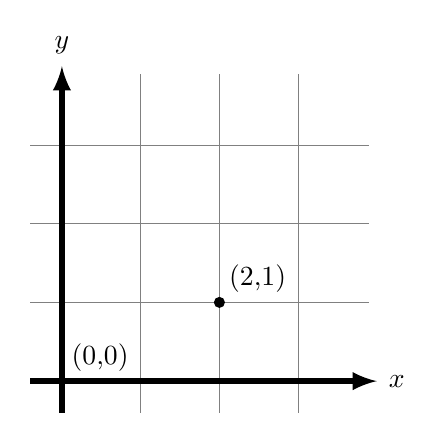
\begin{tikzpicture}
\draw[help lines,step=1cm,very thin](-0.4cm,-0.4cm)grid(3.9cm,3.9cm);
\draw[->,line width=0.7mm](-0.4cm,0)--(4cm,0)node[right]{$x$};
\draw[->,line width=0.7mm](0,-0.4cm)--(0,4cm)node[above]{$y$};
\draw (0,0)node[above right]{(0,0)};
\fill (2cm,1cm)node[above right]{(2,1)}circle(2pt);
\end{tikzpicture}}
\ffigbox{\caption{极坐标表示}\label{fig:jizuobiao1}}{
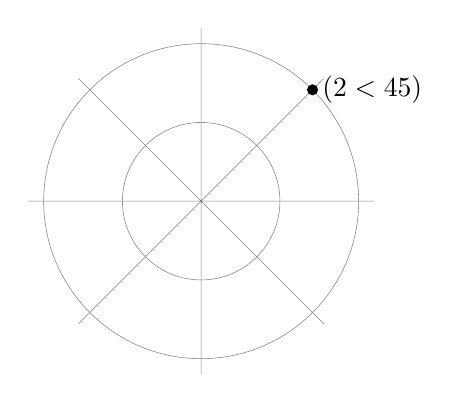
\begin{tikzpicture}
\draw[help lines,very thin](-2.2cm,0)--(2.2cm,0)(0,-2.2cm)--(0,2.2cm)(45:2.2cm)--(225:2.2cm)(135:2.2cm)--(-45:2.2cm);
\draw[help lines,very thin](0,0)circle(1cm)circle(2cm);
\fill (45:2cm)node[right]{$(2<45\degree)$}circle(2pt);
\end{tikzpicture}
}
\end{floatrow}
\end{figure}
\subsubsection{极坐标系}
极坐标系是一个二维坐标系统,它用一段相对于中心点的距离和一个夹角来表示坐标区域中的点,其坐形式为$(\rho,\theta)$,如图\ref{fig:jizuobiao1}所示。其中$\rho$表示距离,永远取正值,$\theta$表示角度,取值范围为$0-360\degree$。
\subsubsection{绝坐标和相对坐标}
绝对坐标是以当前坐标原点为基点进行参照所获得的坐标值。如$(3,5)$,$(4<45\degree)$。

相对坐标是以前面输入的坐标点为参照所获得的坐标值,表示方法是在坐标值前面加一个“@”符号。例如,相对直角坐标表示为$(@5,4)$,相对极坐标表示为$(@5<35)$。

例如,绘制一条两个端点分别为$(3,5)$和$(6,9)$的直线。调用line命令:

\noindent
命令: line 指定第一点: 3,5\\
指定下一点或 [放弃(U)]:\\
用绝对坐标方式输入,$(6,9)$就可以绘出直线。\\
用相对坐标方式输入,可知$(6,9)$相对于$(3,5)$的$X$轴增量为3,$Y$轴增量为4,故输入相对坐标$(@3,4)$也可以绘出直线。

\indent
但是,从AutoCAD的实际绘图过程来看,多种坐标输入方式配合使用会使整个绘图过程更加灵活和方便,再配合目标捕捉和夹点编辑等方式,则使绘图更精确、更快捷。
\subsection{图纸幅面及格式}
\subsubsection{图纸幅面}
“图形界限”中我们所设置的297$\times $210的尺寸就是国家标准中的A4图纸幅面。国家标准《技术制图》中规定幅面的尺寸是为了方便绘制、使用和保管图样。因此,在绘制图样时,应优先采用表\ref{tab:tufubiao1}中规定的尺寸,必要时允许先用规定的加长幅面,加长幅面的尺寸由基本幅面短边的成整数倍增加后得出,如图\ref{fig:tufujiachang}所示。其中粗实细部分为基本幅面。加长后幅面记作:基本幅面代号$\times $倍数。如$A3\times 3$,表示按A3图幅短边加长为297mm的3倍,即加长后图纸尺寸为$420mm\times 891mm$。
%\suppressfloats[t]
\begin{table}[htbp]
\caption{图纸幅面及周边尺寸}\label{tab:tufubiao1}
\begin{tabular}{*{6}{c|}c}
\hline
\multicolumn{2}{c|}{幅面代号}&A0&A1&A2&A3&A4\\ \hline
\multicolumn{2}{c|}{尺寸 $B\times L$}&$841\times 1189$&$594\times 841$&$420\times 594$&$297\times 420$&$210\times 297$\\ \hline
\multirow{3}*{图框}&a&\multicolumn{5}{|c}{25}\\ \cline{2-7}
&c&\multicolumn{3}{|c}{10}&\multicolumn{2}{|c}{5}\\ \cline{2-7}
&e&\multicolumn{2}{|c}{20}&\multicolumn{3}{|c}{10}\\
\hline
\end{tabular}
\end{table}

\begin{figure}[htbp]
\centering
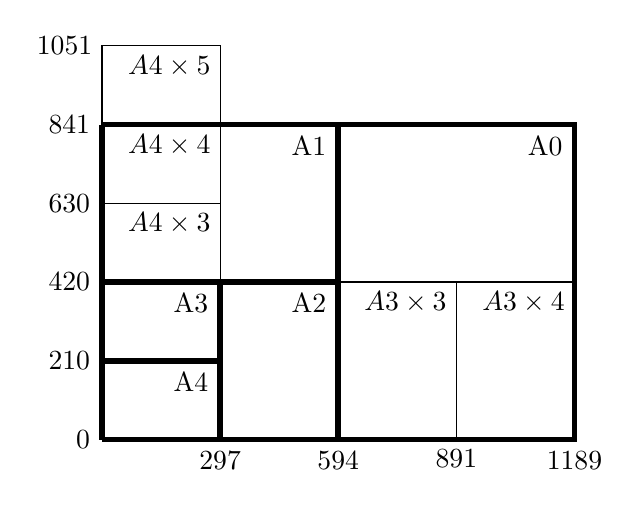
\begin{tikzpicture}
\draw[line width=0.7mm] (0,0)node[left]{0}--(0,1cm)node[left]{210}--(0,2cm)node[left]{420}--(0,3cm)node[left]{630}--(0,4cm)node[left]{841};
\draw(0,4cm)--(0,5cm)node[left]{1051}--(1.5cm,5cm)node[below left]{$A4\times 5$}--(1.5cm,2cm);
\draw[line width=0.7mm](0,1cm)--(1.5cm,1cm)node[below left]{A4}(0,2cm)--(1.5cm,2cm)node[below left]{A3}--(1.5cm,0)node[below]{297};
\draw(0,3cm)--(1.5cm,3cm)node[below left]{$A4\times 3$};
\draw[line width=0.7mm](0,4cm)--(3cm,4cm)node[below left]{A1}--(3cm,0)node[below]{594}(1.5cm,2cm)--(3cm,2cm)node[below left]{A2};
\draw[line width=0.7mm](3cm,4cm)--(6cm,4cm)node[below left]{A0}--(6cm,0)node[below]{1189}--(0,0);
\draw(3cm,2cm)--(4.5cm,2cm)node[below left]{$A3\times 3$}--(6cm,2cm)node[below left]{$A3\times 4$}(4.5cm,2cm)--(4.5cm,0)node[below]{891};
\draw(1.5cm,4cm)node[below left]{$A4\times 4$};
\end{tikzpicture}
\caption{图纸幅面及加长边} \label{fig:tufujiachang}
\end{figure}

从表\ref{tab:tufubiao1}中可以看出幅面之间的关系为:将A0图纸的长边对折后得到两张A1图纸,将A1图纸的长边对折后得到两纸A2图纸,以此类推。

\subsubsection{标题栏}
每张图样上必须画出标题栏,标题栏位于图样的右下角,与看图的方向一致。

标题栏分为更必区、签字区、名称及代号区和其他区,如图\ref{fig:biaotilan}所示。
\tikzset{
>=latex,
center lines/.style={dash pattern=on 20pt off 3pt on 2pt off 3pt},
importance lines/.style={line width=1pt}
}
\noindent
\begin{figure}[htbp]
\begin{tikzpicture}[scale=0.65]
\draw[line width=0.7mm](0,0)rectangle(180mm,56mm);
\draw(0,7mm)--(12mm,7mm)--(40mm,7mm)--++(40mm,0);
\draw(6mm,3.5mm)node{\tiny 工艺};
\draw(46mm,3.5mm)node{\tiny 批准};
\draw(0,14mm)--++(80mm,0);
\draw(6mm,10.5mm)node{\tiny 审核};
\draw(0,21mm)--++(12mm,0)--++(12mm,0)--++(16mm,0)--++(12mm,0)--++(12mm,0)--++(16mm,0);
\draw(6mm,24.5mm)node{\tiny设计};
\draw(18mm,24.5mm)node{\tiny(签名)};
\draw(32mm,24.5mm)node{\tiny(年月日)};
\draw(46mm,24.5mm)node{\tiny标准化};
\draw(58mm,24.5mm)node{\tiny签名};
\draw(72mm,24.5mm)node{\tiny(年月日)};
\draw(12mm,0)--++(0,28mm)(24mm,0)--++(0,28mm)(40mm,0)--++(0,28mm)(52mm,0)--++(0,28mm)(64mm,0)--++(0,28mm)(80mm,0)--++(0,28mm);
\draw(0,28mm)--++(10mm,0)--++(10mm,0)--++(16mm,0)--++(16mm,0)--++(12mm,0)--++(16mm,0);
\draw(5mm,31.5mm)node{\tiny 标记};
\draw(15mm,31.5mm)node{\tiny 处数};
\draw(28mm,31.5mm)node{\tiny 分区};
\draw(44mm,31.5mm)node{\tiny 更改文件号};
\draw(56mm,31.5mm)node{\tiny 签名};
\draw(72mm,31.5mm)node{\tiny 年月日};
\draw(0,35mm)--++(80mm,0)(0,42mm)--++(80mm,0)(0,49mm)--++(80mm,0);
\draw(10mm,28mm)--++(0,28mm)(20mm,28mm)--++(0,28mm)(36mm,28mm)--++(0,28mm)(52mm,28mm)--++(0,28mm)(64mm,28mm)--++(0,28mm)(80mm,28mm)--++(0,28mm);
\draw(80mm,9mm)--++(50mm,0);
\draw(105mm,4.5mm)node{\tiny 共\quad张\quad第\quad张};
\draw(80mm,18mm)--++(26mm,0)--++(12mm,0)--++(12mm,0);
\draw(93mm,23mm)node{\tiny 阶段标记};
\draw(112mm,23mm)node{\tiny 重量};
\draw(124mm,23mm)node{\tiny 比例};
\draw(86.5mm,9mm)--++(0,9mm)(93mm,9mm)--++(0,9mm)(99.5mm,9mm)--++(0,9mm)(106mm,9mm)--++(0,18mm)(118mm,9mm)--++(0,18mm);
\draw(80mm,28mm)--++(50mm,0);
\draw(130mm,0)--++(0,56mm);
\draw(130mm,18mm)--++(50mm,0)(130mm,38mm)--++(50mm,0);
\draw (155mm,9mm)node{\tiny(图样代号)};
\draw(155mm,28mm)node{\tiny(图样名称)};
\draw(155mm,48mm)node{\tiny(单位名称)};
\draw(105mm,48mm)node{\tiny(材料标记)};
\draw[<->](99.5mm,12mm)--(106mm,12mm)node[midway,above]{\tiny 6.5};
\draw(-14mm,0)--(0,0)(-7mm,7mm)--(0,7mm)(-14mm,56mm)--(0,56mm);
\draw[<->](-5mm,0)--(-5mm,7mm)node[midway,above,rotate=90]{\tiny 7};
\draw[<->](-13mm,0)--(-13mm,56mm)node[midway,above,rotate=90]{\tiny $8\times 7(56)$};
\draw(130mm,9mm)--++(9mm,0)(130mm,28mm)--++(9mm,0);
\draw[<->](137mm,0)--++(0,9mm)node[midway,above,rotate=90]{\tiny 9};
\draw[<->](137mm,9mm)--++(0,9mm)node[midway,above,rotate=90]{\tiny 9};
\draw[<->](137mm,18mm)--++(0,10mm)node[midway,above,rotate=90]{\tiny 10};
\draw(180mm,0)--++(9mm,0)(180mm,18mm)--++(9mm,0)(180mm,38mm)--++(9mm,0);
\draw[<->](187mm,0)--++(0,18mm)node[midway,above,rotate=90]{\tiny 18};
\draw[<->](187mm,18mm)--++(0,20mm)node[midway,above,rotate=90]{\tiny 20};
\draw(0,-9mm)--++(0,9mm)(12mm,-9mm)--++(0,9mm)(24mm,-9mm)--++(0,9mm)(40mm,-9mm)--++(0,9mm)(52mm,-9mm)--++(0,9mm)(64mm,-9mm)--++(0,9mm)(80mm,-9mm)--++(0,9mm)(130mm,-9mm)--++(0,9mm);
\draw[<->](0,-7mm)--++(12mm,0)node[midway,above]{\tiny 12};
\draw[<->](12mm,-7mm)--++(12mm,0)node[midway,above]{\tiny 12};
\draw[<->](24mm,-7mm)--++(16mm,0)node[midway,above]{\tiny 16};
\draw[<->](40mm,-7mm)--++(12mm,0)node[midway,above]{\tiny 12};
\draw[<->](52mm,-7mm)--++(12mm,0)node[midway,above]{\tiny 12};
\draw[<->](64mm,-7mm)--++(16mm,0)node[midway,above]{\tiny 16};
\draw[<->](80mm,-7mm)--++(50mm,0)node[midway,above]{\tiny 50};
\draw(0,-18mm)--(0,0)(180mm,-18mm)--(180mm,0);
\draw[<->](0,-16mm)--(180mm,-16mm)node[midway,above]{\tiny 180};
\draw(0,56mm)--++(0,7mm)(10mm,56mm)--++(0,7mm)(20mm,56mm)--++(0,7mm)(36mm,56mm)--++(0,7mm)(52mm,56mm)--++(0,7mm)(64mm,56mm)--++(0,7mm)(80mm,56mm)--++(0,7mm);
\draw[<->](0,61mm)--++(10mm,0)node[midway,above]{\tiny 10};
\draw[<->](10mm,61mm)--++(10mm,0)node[midway,above]{\tiny 10};
\draw[<->](20mm,61mm)--++(16mm,0)node[midway,above]{\tiny 16};
\draw[<->](36mm,61mm)--++(16mm,0)node[midway,above]{\tiny 16};
\draw[<->](52mm,61mm)--++(12mm,0)node[midway,above]{\tiny 12};
\draw[<->](64mm,61mm)--++(16mm,0)node[midway,above]{\tiny 16};
\draw(106mm,28mm)--++(0,7mm)(118mm,28mm)--++(0,7mm);
\draw[<->](80mm,33mm)--++(26mm,0)node[midway,above]{\tiny $4\times 6.5(26)$};
\draw[<->](106mm,33mm)--++(12mm,0)node[midway,above]{\tiny 12};
\draw[<->](118mm,33mm)--++(12mm,0)node[midway,above]{\tiny 12};
\end{tikzpicture}
\caption{标题栏格式及尺寸}\label{fig:biaotilan}
\end{figure}

\begin{figure}[htbp]
\centering
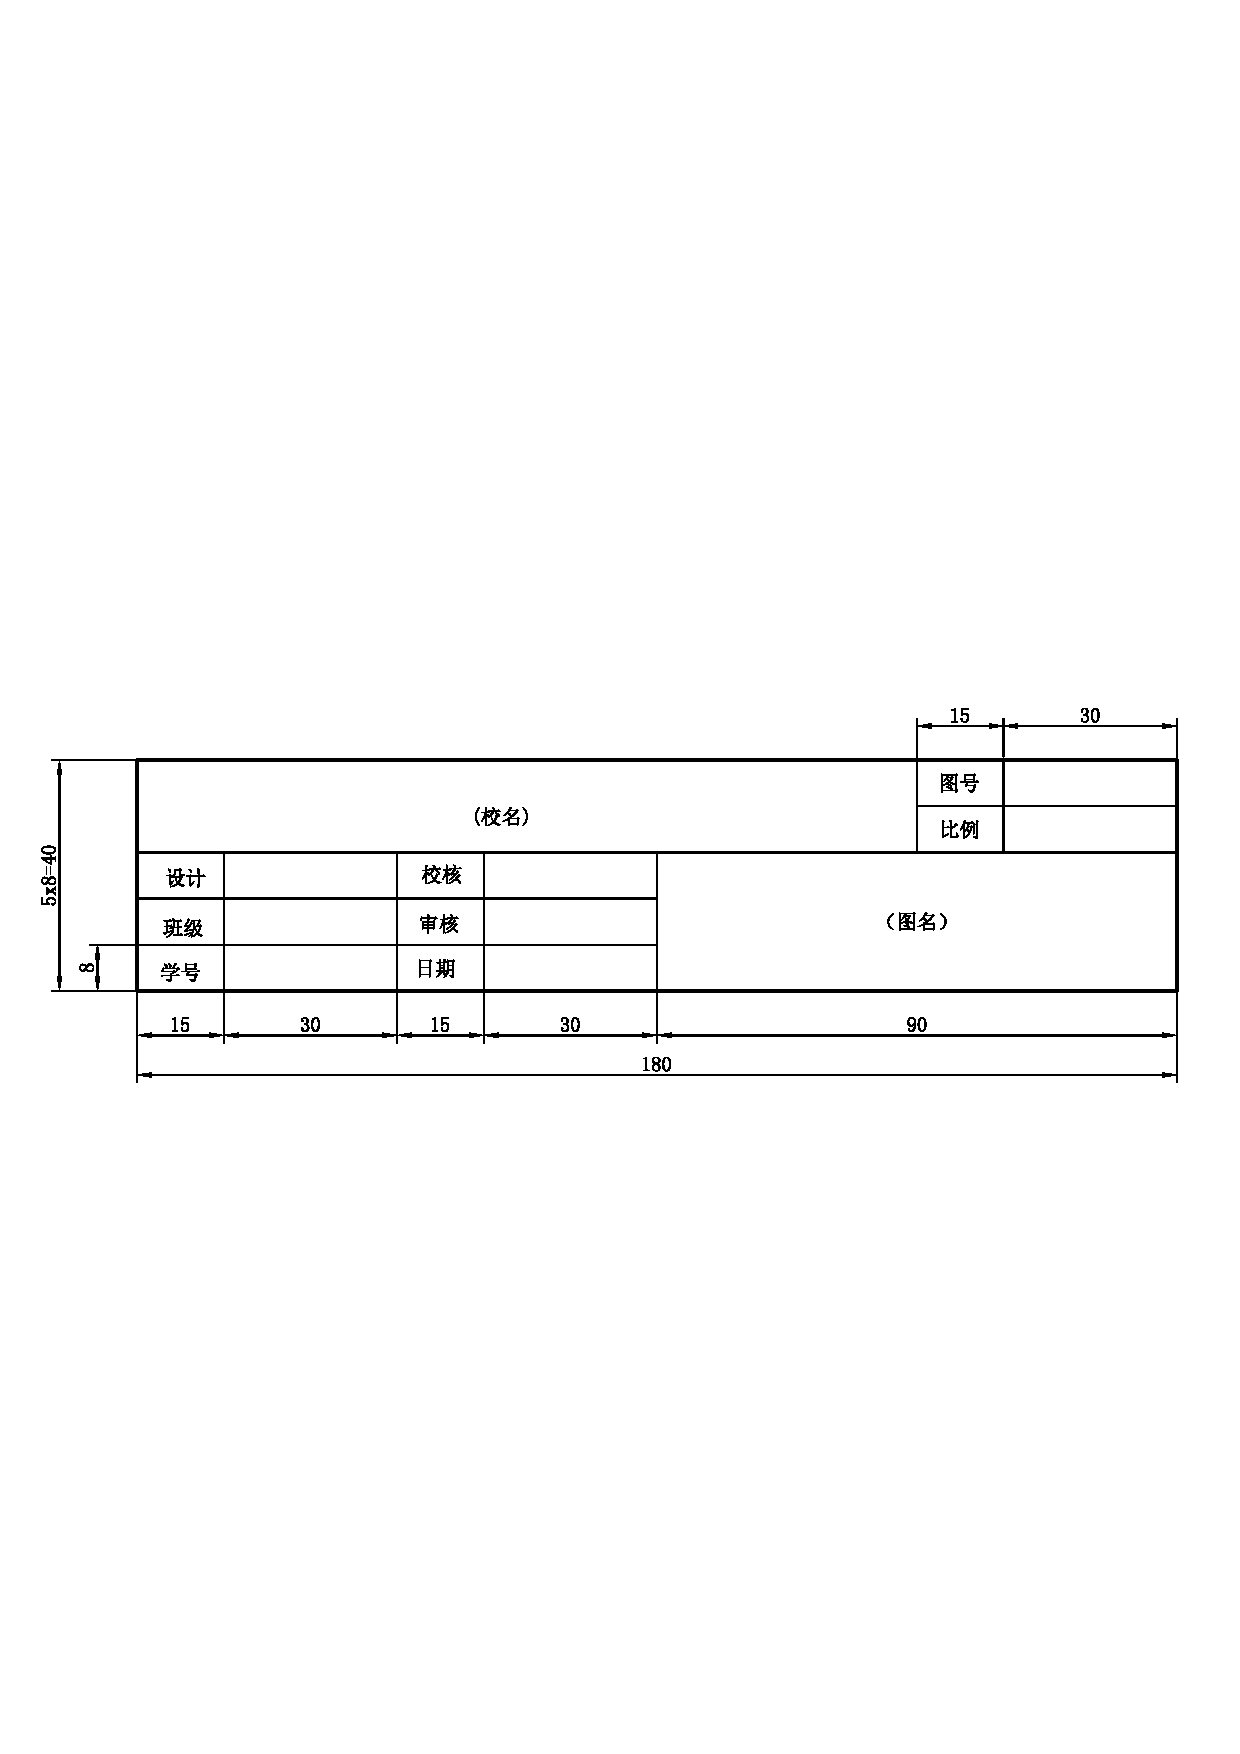
\includegraphics[scale=0.65]{biaotilan.pdf}
\caption{学生用标题栏格式及尺寸}\label{fig:biaotilan1}
\end{figure}
\indent

\subsubsection{图框格式}
图框格式分为留装订边和不留装订边两种,其装订边尺寸如表\ref{tab:tufubiao1}所示。图\ref{fig:zhuangding}所示为采用A4幅面竖装和A3幅面横装时,留装订边和不留装订边的图框格式。
\noindent
\tikzset{
>=latex,
center lines/.style={dash pattern=on 20pt off 3pt on 2pt off 3pt},
importance lines/.style={line width=1pt}
}
\begin{figure}[htbp]
\centering
\subfloat[留装订边格式]{
\begin{tikzpicture}
\draw(0,0)rectangle(4cm,5cm);
\draw[line width=0.7mm](0.5cm,0.25cm)rectangle(3.75cm,4.75cm)(1.5cm,0.25cm)--(1.5cm,1cm)--(3.75cm,1cm)node[midway,below]{标题栏};
\draw(-0.7cm,0)--(0,0)(-0.7cm,5cm)--(0cm,5cm);
\draw[<->](-0.5cm,0)--(-0.5cm,5cm)node[midway,above,rotate=90]{$L$};
\draw(0,-0.7cm)--(0,0)(4cm,-0.7cm)--(4cm,0);
\draw[<->](0,-0.5cm)--(4cm,-0.5cm)node[midway,above]{$B$};
\draw[->](1cm,-0.45cm)--(1cm,0);
\draw[->](1cm,0.65cm)--(1cm,0.25cm)node[midway,above,rotate=90]{$c$};
\draw(1cm,0)--(1cm,0.25cm);
\draw[->](-0.4cm,2cm)--(0,2cm);
\draw[->](0.9cm,2cm)--(0.5cm,2cm);
\draw(0,2cm)--(0.5cm,2cm)node[midway,above]{$a$};
\draw[->](2cm,5cm)--(2cm,4.35cm)--(2cm,4.75cm);
\draw[->](2cm,5.45cm)--(2cm,5cm)node[midway,above,rotate=90]{$c$};
\draw[->](4cm,2.5cm)--(3.3cm,2.5cm)--(3.75cm,2.5cm);
\draw[->](4.45cm,2.5cm)--(4cm,2.5cm)node[midway,above]{$c$};

\begin{scope}[xshift=5.5cm]
\draw(0,0)rectangle(7cm,5cm);
\draw[line width=0.7mm](0.5cm,0.25cm)rectangle(6.75cm,4.75cm)(4.5cm,0.25cm)--(4.5cm,1cm)--(6.75cm,1cm)node[midway,below]{标题栏};
\draw(-0.7cm,0)--(0,0)(-0.7cm,5cm)--(0cm,5cm);
\draw[<->](-0.5cm,0)--(-0.5cm,5cm)node[midway,above,rotate=90]{$B$};
\draw(0,-0.7cm)--(0,0)(7cm,-0.7cm)--(7cm,0);
\draw[<->](0,-0.5cm)--(7cm,-0.5cm)node[midway,above]{$L$};
\draw[->](3cm,-0.45cm)--(3cm,0);
\draw[->](3cm,0.65cm)--(3cm,0.25cm)node[midway,above,rotate=90]{$c$};
\draw(3cm,0)--(3cm,0.25cm);
\draw[->](-0.4cm,2cm)--(0,2cm);
\draw[->](0.9cm,2cm)--(0.5cm,2cm);
\draw(0,2cm)--(0.5cm,2cm)node[midway,above]{$a$};
\draw[->](3.5cm,5cm)--(3.5cm,4.35cm)--(3.5cm,4.75cm);
\draw[->](3.5cm,5.45cm)--(3.5cm,5cm)node[midway,above,rotate=90]{$c$};
\draw[->](7cm,2.5cm)--(6.3cm,2.5cm)--(6.75cm,2.5cm);
\draw[->](7.45cm,2.5cm)--(7cm,2.5cm)node[midway,above]{$c$};
\end{scope}
\end{tikzpicture}}

\subfloat[不留装订边格式]{
\begin{tikzpicture}
\draw(0,0)rectangle(4cm,5cm);
\draw[line width=0.7mm](0.25cm,0.25cm)rectangle(3.75cm,4.75cm)(1.5cm,0.25cm)--(1.5cm,1cm)--(3.75cm,1cm)node[midway,below]{标题栏};
\draw(-0.7cm,0)--(0,0)(-0.7cm,5cm)--(0cm,5cm);
\draw[<->](-0.5cm,0)--(-0.5cm,5cm)node[midway,above,rotate=90]{$L$};
\draw(0,-0.7cm)--(0,0)(4cm,-0.7cm)--(4cm,0);
\draw[<->](0,-0.5cm)--(4cm,-0.5cm)node[midway,above]{$B$};
\draw[->](1cm,-0.45cm)--(1cm,0);
\draw[->](1cm,0.65cm)--(1cm,0.25cm)node[midway,above,rotate=90]{$c$};
\draw(1cm,0)--(1cm,0.25cm);
\draw[->](-0.4cm,2cm)--(0,2cm);
\draw[->](0.65cm,2cm)--(0.25cm,2cm)node[midway,above]{$c$};
\draw(0,2cm)--(0.25cm,2cm);
\draw[->](2cm,5cm)--(2cm,4.35cm)--(2cm,4.75cm);
\draw[->](2cm,5.45cm)--(2cm,5cm)node[midway,above,rotate=90]{$c$};
\draw[->](4cm,2.5cm)--(3.3cm,2.5cm)--(3.75cm,2.5cm);
\draw[->](4.45cm,2.5cm)--(4cm,2.5cm)node[midway,above]{$c$};

\begin{scope}[xshift=5.5cm]
\draw(0,0)rectangle(7cm,5cm);
\draw[line width=0.7mm](0.25cm,0.25cm)rectangle(6.75cm,4.75cm)(4.5cm,0.25cm)--(4.5cm,1cm)--(6.75cm,1cm)node[midway,below]{标题栏};
\draw(-0.7cm,0)--(0,0)(-0.7cm,5cm)--(0cm,5cm);
\draw[<->](-0.5cm,0)--(-0.5cm,5cm)node[midway,above,rotate=90]{$B$};
\draw(0,-0.7cm)--(0,0)(7cm,-0.7cm)--(7cm,0);
\draw[<->](0,-0.5cm)--(7cm,-0.5cm)node[midway,above]{$L$};
\draw[->](3cm,-0.45cm)--(3cm,0);
\draw[->](3cm,0.65cm)--(3cm,0.25cm)node[midway,above,rotate=90]{$c$};
\draw(3cm,0)--(3cm,0.25cm);
\draw[->](-0.4cm,2cm)--(0,2cm);
\draw[->](0.65cm,2cm)--(0.25cm,2cm)node[midway,above]{$c$};
\draw(0,2cm)--(0.25cm,2cm);
\draw[->](3.5cm,5cm)--(3.5cm,4.35cm)--(3.5cm,4.75cm);
\draw[->](3.5cm,5.45cm)--(3.5cm,5cm)node[midway,above,rotate=90]{$c$};
\draw[->](7cm,2.5cm)--(6.3cm,2.5cm)--(6.75cm,2.5cm);
\draw[->](7.45cm,2.5cm)--(7cm,2.5cm)node[midway,above]{$c$};
\end{scope}
\end{tikzpicture}}
\caption{图框格式}\label{fig:zhuangding}
\end{figure}
\indent

\subsection{正投影法}
\subsubsection{投影}
物体在阳光或灯光下所生的具有影子就称为投影。由于影子只显示了物体的外部轮廓,不能够体现物体内外细节,不具备工程实际价值。在工程实际中,采用不同的线型将物体的内外空间几何元素加以抽像,使之能够具体地反映物体的内外细节,从而形成比较完备的、实用的投影法。投影法主要分为中心投影法和平行投影法两类。
\subsubsection{平行投影法}
中心投影法的所有投影线都不是平行的,主要用于绘制效果比较逼真的建筑或产品立体图,故在此不作讲解,有兴趣的读者可查阅相关书籍深入学习。

图\ref{pingxingtouyin}所示即为平行投影法,从图中可以看出,平行投影法是将光源置于无穷远处,使所有的投影线之间为平行关系的一种投影方法。若投影线与投影面垂直称为正投影法;若投影线与投影面倾斜的称之为斜投影法。平行投影法中,正投影法主要应用于工程图样的绘,斜投影主要用于绘制立体图形。
\begin{figure}[htbp]
\centering
\subfloat[斜投影法]{\label{fig:xietouyinfa}
\begin{tikzpicture}
\draw(0,0)--(30mm,0)--++(30:30mm)--++(-30mm,0)--cycle;
\begin{scope}[xshift=10mm]
\draw[line width=0.4mm](0,0)++(30:10mm)coordinate(a1)--++(10mm,0) coordinate(a2)--++(30:10mm) coordinate(a3)--++(-10mm,0) coordinate(a4)--cycle;
\draw(a1)--++(75:30mm)coordinate(b1) (a2)--++(75:30mm)coordinate(b2) (a3)--++(75:30mm)coordinate(b3) (a4)--++(75:30mm)coordinate(b4);
\draw[line width=0.4mm]($(a1)!.8!(b1)$)--($(a2)!.8!(b2)$)--($(a3)!.8!(b3)$)--($(a4)!.8!(b4)$)--cycle;
\end{scope}
\end{tikzpicture}
}
\subfloat[正投影法]{\label{fig:zhentouyinfa}
\begin{tikzpicture}
\draw(0,0)--(30mm,0)--++(30:30mm)--++(-30mm,0)--cycle;
\begin{scope}[xshift=10mm]
\draw[line width=0.4mm](0,0)++(30:10mm)coordinate(a1)--++(10mm,0) coordinate(a2)--++(30:10mm) coordinate(a3)--++(-10mm,0) coordinate(a4)--cycle;
\draw(a1)--++(0,30mm)coordinate(b1) (a2)--++(0,30mm)coordinate(b2) (a3)--++(0,30mm)coordinate(b3) (a4)--++(0,30mm)coordinate(b4);
\draw[line width=0.4mm]($(a1)!.8!(b1)$)--($(a2)!.8!(b2)$)--($(a3)!.8!(b3)$)--($(a4)!.8!(b4)$)--cycle;
\end{scope}
\end{tikzpicture}
}
\caption{平行投影法}\label{pingxingtouyin}
\end{figure}

\subsubsection{三视图的形成}
根据《工程制图》国家标准,将位于观察者和投影面之间的物体,按照正投影法向投影面进行投影所得的图形称之为视图。从图\ref{fig:singleprojection}中,我们可以看出同一个视图可表示不同的物体,因此工程实际中仅用一个视图很难将物体的大小形状完整清晰的表达出来。通常情况下,需要将物体向多个投影面进行投影才能够完整地表达出物体上下、左右、前后各部分的形状和大小。实际中,经常将物体向三个方向进行投影,形成三个视图,称为三视图。

\begin{figure}[htbp]
\centering
\begin{tikzpicture}
\draw[line width=0.4mm](0,0)coordinate(a1)--(0,5mm)coordinate(a2)--++(30:5mm) coordinate(a3)--++(0,5mm)coordinate(a4)--++(30:5mm) coordinate(a5)--++(0,-10mm)coordinate(a6)--cycle;
\draw[line width=0.4mm](a1)--++(150:10mm)coordinate(a7)--++(0,10mm) coordinate(a8)--++(-30:5mm)coordinate(a9)--++(0,-5mm) coordinate(a10)--(a2);
\draw[line width=0.4mm](a10)--++(30:5mm)--++(0,5mm)(a3)--++(150:5mm)(a4)--++(150:5mm)--++(30:-5mm)(a5)--++(150:10mm)--++(30:-10mm);
\draw[line width=0.4mm](a7)++(150:12mm)coordinate(b1)--++(0,5mm)coordinate(b2)--++(30:5mm) coordinate(b3)--++(0,5mm)coordinate(b4)--++(30:5mm) coordinate(b5)--++(0,-10mm)coordinate(b6)--cycle;
\begin{scope}
\clip (a8)rectangle($(a8)+(-2mm,2mm)$);
\draw(a6)--(b6);
\end{scope}
\draw[line width=0.4mm](b1)--++(150:10mm)coordinate(b7)--++(0,10mm)--++(-30:5mm)--(b2);
\draw[line width=0.4mm](b5)--++(150:10mm)--++(30:-10mm) (b4)--++(150:5mm)coordinate(b8)--++(30:-5mm)(b8)--(b3);
\draw[line width=0.4mm](b7)++(150:15mm)coordinate(c1)--++(0,5mm)coordinate(c2)--++(30:5mm) coordinate(c3)--++(0,5mm)coordinate(c4)--++(30:5mm) coordinate(c5)--++(0,-10mm)coordinate(c6)--cycle;
\draw[line width=0.4mm](c2)--++(0,5mm)coordinate(c7)--(c4);
\begin{scope}
\clip ($(b7)+(0,10mm)$) coordinate(c8)rectangle($(c8)+(-2mm,2mm)$);
\draw(b6)--(c6);
\end{scope}
\draw(a1)--(c1)(a2)--(c2)(a4)--(c4)(a5)--(c5)(a9)--(c7);
\begin{scope}
\draw($(c1)+(30:-10mm)+(0,-3mm)$)--++(0,20mm)--++(30:30mm)--++(0,-20mm)--cycle;
\end{scope}
\end{tikzpicture}
\caption{一个投影面不能确定物体在空间中的形状和位置}\label{fig:singleprojection}
\end{figure}

根据国家标准规定,选三个相互垂直的投影面构成三投影面体系,如图\ref{fig:threeviewprojection}所示。在三视图投影体系中,正对观者的投影面称为正平面,用$V$表示。水平放置的投影面称水平面,用$H$表示。侧立的投影面称为侧平面,用$W$表示。
\begin{figure}[htbp]
\centering
\subfloat[物体在三面投影中的投影]{\label{fig:threeviewprojection}
\begin{tikzpicture}
\begin{scope}[scale=0.5]
\draw[line width=0.4mm](0,0)coordinate(a1)--(0,10mm)coordinate(a2)--++(0:10mm) coordinate(a3)--++(0,10mm)coordinate(a4)--++(0:10mm) coordinate(a5)--++(0,-20mm)coordinate(a6)--cycle;
\draw[line width=0.4mm](a1)--++(135:10mm)coordinate(a7) 
(a2)--++(135:10mm)coordinate(a8) (a3)--++(135:10mm)coordinate(a9) (a4)--++(135:10mm)coordinate(a10)(a5)--++(135:10mm)coordinate(a11);
\draw[line width=0.4mm](a7)--(a8)--(a9)--(a10)--(a11);
\draw(a1)--++(0,-15mm)coordinate(b1);
\draw[line width=0.4mm](b1)--++(135:10mm)coordinate(b2)--++(0:20mm) coordinate(b3)--++(135:-10mm)coordinate(b4)--cycle;
\draw[line width=0.4mm](b1)++(0:10mm)coordinate(b5)--++(135:10mm);
\draw(a7)--++(135:20mm)coordinate(c1);
\draw[line width=0.4mm](c1)--++(0,10mm) coordinate(c2)--++(0:10mm) coordinate(c3)--++(0,10mm) coordinate(c4)--++(0:10mm) coordinate(c5)--++(0,-20mm) coordinate(c6)--cycle;
\draw(a6)--++(0:15mm)coordinate(d1);
\draw[line width=0.4mm](d1)--++(0,20mm)coordinate(d2)--++(135:10mm) coordinate(d3)--++(0,-20mm)coordinate(d4)--cycle;
\draw[line width=0.4mm](d1)++(0,10mm)coordinate(d5)--++(135:10mm);

\draw($(b2)+(135:20mm)+(-15mm,0)$)coordinate(e1)--++(0,50mm)coordinate(e2);
\draw(e1)--++(135:-45mm)coordinate(e3);
\begin{scope}
\clip(a1)--++(135:10mm)--++(-40mm,0)--++(135:-10mm)--cycle;
\draw(e1)--++(50mm,0)coordinate(e4);
\end{scope}
\draw(e2)--++(50mm,0)coordinate(e5);
\draw(e3)--++(50mm,0)coordinate(e6);
\begin{scope}
\clip(a5)--(a11)--++(0,35mm)--++(135:-10mm)--cycle;
\draw(e4)--(e5);
\end{scope}
\begin{scope}
\clip(a6)--++(0,-35mm)--++(40mm,0)--++(0,35mm)--cycle;
\draw(e6)--(e4);
\end{scope}
\draw(e6)--++(0,50mm)coordinate(e7)--(e5);
\draw(a8)--(c2)(a9)--(c3)(a10)--(c4)(a11)--(c5)(a7)--(b2)(a3)--(b5)(a6)--(b4)(a3)--(d5)(a5)--(d2)(a11)--(d3);
\draw(e2)++(1mm,-3mm)node[below,right]{\tiny $V$ 主视图};
\draw(e3)++(1mm,2mm)node[below,right]{\tiny $H$ 俯视图};
\draw(e7)++($(135:25mm)+(0,-3mm)$)node[below,right,rotate=-45]{\tiny 左视图 $W$};
\draw[->,line width=0.3mm](e1)++(10mm,-15mm)node[left]{\tiny 左视方向}--++(10mm,0);
\draw[->,line width=0.3mm](e6)++(-15mm,-3mm)node[below,sloped]{\tiny 主视方向}--++(135:10mm);
\draw[->,line width=0.3mm](e5)++(-15mm,5mm)node[above]{\tiny 俯视方向}--++(0,-10mm);
\end{scope}
\end{tikzpicture}}
\subfloat[三个投影面的展开]{\label{fig:threeviewzhankai}
\begin{tikzpicture}
\begin{scope}[scale=0.45]
\draw(0,0)coordinate(a1)--++(0,50mm) coordinate(a2)--++(50mm,0) coordinate(a3)--++(0,-50mm) coordinate(a4)--cycle;
\draw(a1)--++(-50:50mm)coordinate(a5)--++(50mm,0) coordinate(a6)--(a4);
\draw(a3)--++(-40:50mm)coordinate(a7)--++(0,-50mm) coordinate(a8)--(a4);
\draw[line width=0.4mm](a1)++(15mm,15mm)coordinate(b1)--++(20mm,0)coordinate(b2) --++(0,20mm)coordinate(b3)--++(-10mm,0)--++(0,-10mm)--++(-10mm,0)--cycle;
\draw(b1)--++(0,-15mm)coordinate(b4)(b2)--++(0,-15mm)(b2)--++(15mm,0)coordinate(b5)(b3)--++(15mm,0);
\draw(b4)--++(-50:20mm)coordinate(c1);
\draw[line width=0.4mm](c1)--++(20mm,0)coordinate(c2)--++(-50:10mm)--++(-20mm,0)--cycle;
\draw[line width=0.4mm]($(c1)+(10mm,0)$)--++(-50:10mm);
\draw(c2)--++(-50:-20mm);
\draw(b5)--++(-40:20mm)coordinate(d1);
\draw[line width=0.4mm](d1)--++(0,20mm)coordinate(d2)--++(-40:10mm)--++(0,-20mm)--cycle;
\draw[line width=0.4mm](d1)++(0,10mm)--++(-40:10mm);
\draw(d2)--++(-40:-20mm);
\draw(a2)++(1mm,-3mm)node[below,right]{\tiny $V$ 主视图};
\draw(a5)++(1mm,2mm)node[below,right]{\tiny $H$ 俯视图};
\draw(a7)++($(-40:-25mm)+(0,-3mm)$)node[below,right,rotate=-40]{\tiny 左视图 $W$};
\draw[->,line width=0.3mm](a5)arc(-50:-80:20mm);
\draw[->,line width=0.3mm](a7)arc(-40:-10:20mm);
\end{scope}
\end{tikzpicture}}

\subfloat[展开后的三视图]{\label{fig:threeview}
\begin{tikzpicture}
\begin{scope}[scale=0.4]
\draw(0,-50mm)--(0,50mm)--++(100mm,0)--++ (0,-50mm)--++(-50mm,0)--++(0,-50mm)--cycle;
\draw(0,0)--++(50mm,0)--++(0,50mm);
\draw[line width=0.4mm](15mm,15mm)--++(20mm,0)--++(0,20mm)--++(-10mm,0) --++(0,-10mm)--++(-10mm,0)--cycle;
\draw[line width=0.4mm](70mm,15mm)--++(0,20mm)--++(10mm,0)--++(0,-20mm)--cycle;
\draw[line width=0.4mm](70mm,25mm)--++(10mm,0);
\draw[line width=0.4mm](15mm,-20mm)--++(20mm,0)--++(0,-10mm)--++(-20mm,0)--cycle;
\draw[line width=0.4mm](25mm,-20mm)--++(0,-10mm);
\draw(0,50mm)++(1mm,-3mm)node[below,right]{\tiny $V$ 主视图};
\draw(0,-50mm)++(1mm,2mm)node[below,right]{\tiny $H$ 俯视图};
\draw(100mm,50mm)++(-29mm,-4mm)node[below,right]{\tiny 左视图 $W$};
\end{scope}
\end{tikzpicture}}
\subfloat[三视图投影规律]{\label{fig:threeviewguilu}
\begin{tikzpicture}
\begin{scope}[scale=0.6]
\draw[line width=0.4mm](0,0)coordinate(a1)--++ (20mm,0)coordinate(a2)--++ (0,20mm)coordinate(a3)--++ (-10mm,0)coordinate(a4)--++(0,-10mm)coordinate(a5)--++ (-10mm,0)coordinate(a6)--cycle;
\draw(a4)node[above]{\tiny 上};
\draw(a4)++(0,-20mm)node[below]{\tiny 下};
\draw(a6)node[left]{\tiny 左};
\draw(a2)++(0,10mm)node[right]{\tiny 右};
\draw[line width=0.4mm](a1)++(0,-25mm)coordinate(b1)--++(0,-10mm) coordinate(b2)--++(20mm,0)coordinate(b3)--++(0,10mm) coordinate(b4)--cycle;
\draw[line width=0.4mm](b1)++(10mm,0)node[above]{\tiny 后}--++(0,-10mm)node[below]{\tiny 前};
\draw(a1)--(b1)(a2)--(b4);
\draw[<->]($(a1)!.6!(b1)$)--($(a2)!.6!(b4)$)node[midway,above]{\tiny 长对正};
\draw[line width=0.4mm](a2)++(25mm,0)coordinate(c1)--++(10mm,0)coordinate(c2)--++(0,20mm) coordinate(c3)--++(-10mm,0)coordinate(c4)--cycle;
\draw[line width=0.4mm](c1)++(0,10mm)node[left]{\tiny后}--++(10mm,0)node[right]{\tiny前};
\draw(a2)--(c1)(a3)--(c4);
\draw[<->]($(a2)!.6!(c1)$)--($(a3)!.6!(c4)$)node[midway,above,sloped]{\tiny高平齐};
\draw(b3)--++(10mm,0)coordinate(d1);
\draw(b4)--++(10mm,0)coordinate(d2);
\draw[<->]($(b3)!.8!(d1)$)coordinate(d3)--($(b4)!.8!(d2)$)coordinate(d4);
\draw(c1)--++(0,-10mm)coordinate(d5);
\draw(c2)--++(0,-10mm)coordinate(d6);
\draw[<->]($(c1)!.8!(d5)$)coordinate(d7)--($(c2)!.8!(d6)$)coordinate(d8);
\draw($(d4)!.4!(d3)$)coordinate(d9)--($(d7)!.4!(d8)$)coordinate(d10);
\draw($(d9)!.5!(d10)$)--++(6mm,0)node[right]{\tiny宽相等};
\end{scope}
\end{tikzpicture}}
\caption{三视图的形成及投影规律}
\end{figure}

接下来,将物体由前向后投影所得的$V$面视图称为主视;将物体由上向下投影所得的$H$面视图称为府视图;将物体由左向右投影所得的$W$面视图称为左视图。最后,按照国家标准,以图\ref{fig:threeviewzhankai}所示方式进行展开,也不是以$V$面视图为基准,$H$面绕$V$面与$H$面的交线所形成的$X$轴向下旋转$90\degree$;$W$面绕$V$面与$W$面的交线所形成的$Z$轴向右旋转$90\degree$,使$V$、$H$、$W$面处于同一个平面内,如图\ref{fig:threeview}所示。展开后的三视图既不需要画边框和投影轴,也不需要标视图名称,如图\ref{fig:threeviewguilu}所示。
\subsubsection{三视图投影规律}
从图\ref{fig:threeviewguilu}中,我们可以得出:主视图反映物体的上下和左右关系,即反映物体的长和高;俯视图反映物体的左右和前后关系,即反映物体的长和宽;左视图反映物体的上下和前后,即反映物体的高和宽。因此,三视图的投影规律为:
\begin{itemize}
\item 主、俯视图长对正;
\item 主、左视图高平齐;
\item 俯、左视图宽相等。
\end{itemize}

三视图的投影规律不仅适用于物体整体之间的投影,也适用于空间中的点、线面。同时它也是画图和读图的基础规则。
